
\documentclass[
  english,        % define the document language (english, german)
  font=times,     % define main text font (helvet, times, palatino, libertine)
  onecolumn,      % use onecolumn or twocolumn layout
]{tumarticle}


% load additional packages
\usepackage{lipsum}
\usepackage{csquotes}
\usepackage[style=numeric-comp,sorting=none]{biblatex}
\usepackage{graphicx}
\usepackage{amsmath}
\usepackage{subcaption}

\addbibresource{resources/literature.bib}


% article metadata
\title{Time stepping review of open-source solvers}
\subtitle{Guided research}

\author[email=marc.amoros@tum.de]{Marc Amorós}

\date{
    \small
    \textbf{Advisor:} M.Sc. Benjamin Rodenberg \\
    \textbf{Supervisor:} Prof. Dr. Hans-Joachim Bungartz \\
}

\begin{document}

\maketitle

% \begin{abstract}
%   This is a short abstract summarizing the main points of your article.
% \end{abstract}

\section{Introduction}
\begin{itemize}
    \item Introduction to coupling simulations (FSI) and to the preCICE library. 
    \item Some brief motivation of performing a convergence study on the known solvers.
    \item Talk somehow about higer timestepping schemes, and why/when is good to use them. Should you use a higher order timestepping scheme if it doesn't give good results? (No bc it is slower) 
    \item Say why we chose this two open source solvers.
    \item Explain difference between preCICEv2 and preCICEv3.
\end{itemize}


\section{OpenFOAM}
\begin{itemize}
    \item Small introduction to OpenFOAM.
    \item Explain time stepping schemes available in the solver, and their orders. Mainly talk about Euler method, and Crank Nikolson, as they are the two cases we used.
    \item Talk about the script created to automatize the procedure of running these simulations. 
\end{itemize}

OpenFOAM is an open-source computational fluid dynamics (CFD) software package widely used for simulating and analyzing complex fluid flow problems. Its solver modules employ finite volume methods to numerically solve the Navier-Stokes equations, making it a versatile tool for simulating fluid dynamics in various engineering and scientific applications. In this solver we can find various time stepping schemes, and we focused in two for our analysis. The first one is the Euler implicit scheme, as is usually the default one. Given the following partial differential equation:

\begin{equation}
    \frac{\partial u}{\partial t} = F(u, x, t)
\end{equation}

The Euler implicit scheme would discretize it as follows:

\begin{equation}
    \frac{u_i^{n+1} - u_i^n}{\Delta t} = {F_i}^{n+1}(u, x, t)
\end{equation}

This is a first order method, that is quite stable, reason why it is usually the default choice. For the purpouse of this study, we also chose a second order scheme, this being the Crank Nikolson method \cite{crank1947practical}. This scheme is a combination of an explicit and an implicit Euler step, leading to a second order convergence in time. This method would discretize the previous PDE as: 

\begin{equation}
    \frac{u_i^{n+1} - u_i^n}{\Delta t} = \frac{1}{2} \left[{F_i}^{n}(u, x, t) +  {F_i}^{n+1}(u, x, t) \right]
\end{equation}


OpenFOAM uses a sligtly different version of this method, by introducing a blending coefficient $\theta$ between the Euler implicit method and the Crank Nikolson method. If $\theta = 0$ then we obtain the implicit Euler method, and if $\theta = 1$ then it's Crank Nikolson. For stability, the value $\theta = 0.9$ is recomended in their documentation.

\begin{equation}
    \frac{u_i^{n+1} - u_i^n}{\Delta t} = \frac{\theta}{2} {F_i}^{n}(u, x, t) + \left( 1 - \frac{\theta}{2} \right) {F_i}^{n+1}(u, x, t)
\end{equation}

 TODO:(include this?) Diffusion example of Crank Nikolson.
\begin{equation}
    \frac{u_i^{n+1} - u_i^{n}}{\Delta t} = \frac{u_{i + 1}^{n} - 2u_{i}^{n} + u_{i - 1}^{n}}{2 \left( \Delta x \right)^2} +  \frac{u_{i + 1}^{n + 1} - 2u_{i}^{n + 1} + u_{i - 1}^{n + 1}}{2 \left( \Delta x \right)^2}
\end{equation}


\subsection{Solver parameters}
\begin{itemize}
    \item Talk about the important parameters in the configuration, to obtain accurately enough results, as those where quite time consuming to find. For example, foamToVTK is not accurate enough, and was misleading at the beginning. Also mention the solver used.
\end{itemize}

\subsection{Case study: Taylor–Green vortex}

To study the convergence behaviour of the OpenFOAM, we focused on the Taylor-Green vortex \cite{taylor1937mechanism, chorin1968numerical}, a standard setup in CFD for the validation of fluid flow solvers, given that an analytical solution of the case is known. In a 2D, this solution can be obtained by the formulas:
\begin{align}
    &u(x, y, t) = -\cos(x) \sin(y) e^{-2\nu t} \\
    &v(x, y, t) = \sin(x) \cos(y) e^{-2\nu t} \\
    &p(x, y, t) = -\frac{1}{4}\left[\cos(2x) + \sin(2y)\right]e^{-2\nu t}
\end{align}
where $u$ and $v$ are the horizontal and vertical velocities respectively, $p$ is the pressure and $\nu$ is the viscosity of the fluid. This solution holds for a square domain of size $2\pi$. 
We implemented a program that computes the initial velocity for this setup, and writes it into the OpenFOAM configuration. We also wrote a script to automatize the configuration and execution of different setups with varying parameters, so we can perform several experiments automatically.
To observe the behaviour of the error, we did several executions of our setup case, fixing all the parameters (grid size, initial velocity, solver tolerances etc.) and changing the time-step size. On our analysis, we mainly focused on the velocity profile.

In a simulation, there are several elements that contribute to the error $\varepsilon_{u}$. In this study, we were only interested in the error contribution of the time discretization scheme $\varepsilon_{\Delta t}$ to verify the order of the scheme. We assume that the error is formed by $\varepsilon_u = \varepsilon_{\Delta t} + \varepsilon_{\Delta x} + \varepsilon_\text{num}$, where $\varepsilon_{\Delta x}$ is the spatial discretization error, and $\varepsilon_\text{num}$ is the error introduced by numerical errors, and other factors. We know that $\varepsilon_{\Delta x}$ is related to the grid size, so we can assume that is constant among the experiments with the same grid size.

\begin{figure}[!htbp]
    \centering
    \begin{subfigure}[b]{0.49\textwidth}
      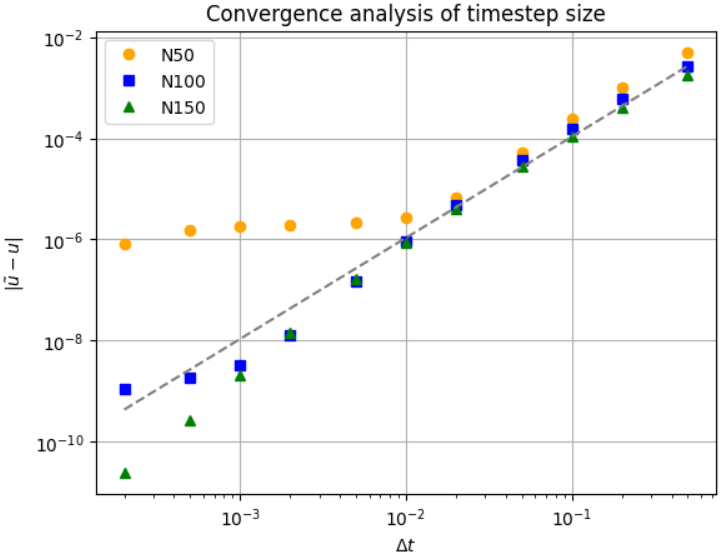
\includegraphics[width=\textwidth]{resources/convergence_study_openfoam.png}
      \caption{}
      \label{fig:convergence_openfoam}
    \end{subfigure}
    \hspace{1pt}
    \begin{subfigure}[b]{0.49\textwidth}
      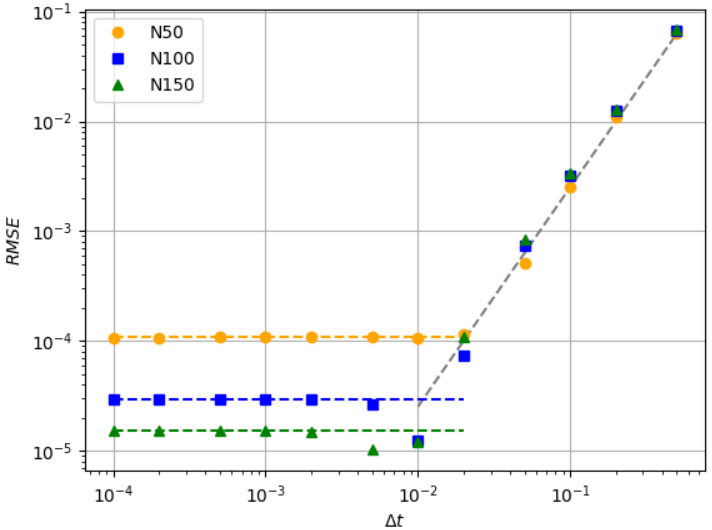
\includegraphics[width=\textwidth]{resources/RMSE_study.png}
      \caption{}
      \label{fig:RMSE_openfoam}
    \end{subfigure}
    \caption{Caption for both figures}
    \label{fig:figures}
  \end{figure}
  


There are several possible approaches to study the error. Our strategy was to choose a position cell $(i,j)$ and compare the values of the cell in this position for the different samples. We define as the reference sample $\tilde{u}$, obtained by running the simulation with a $\Delta t = 10^{-5}$. 
We computed the absolute difference between every sample and the chosen reference solution $|u - \tilde{u}|$ and we plotted them in Figure \ref{fig:convergence_openfoam}, for three different grid sizes. As we assumed that $\varepsilon_{\Delta x}$ is constant among the samples with the same grid size, in this plot we obtain $\varepsilon_{\Delta t} + \varepsilon_\text{num}$, allowing us to extract conclusions form the convergence behaviour of $\varepsilon_{\Delta t}$. We can observe how the error decreases when the timestep gets smaller, proportionally to $\text{O}(\Delta t^2)$, until a point where the error flattens. Our assumption is that this happens when $\varepsilon_{\Delta t} < \varepsilon_\text{num}$, and after a certain point this $\varepsilon_\text{num}$ dominates the entire error. It is also remarkable to see how this point of flattening happens on smaller timesteps for increasing resolutions of the domain.

As me mentioned before, the Taylor–Green vortex scenario has an analytical solution $u^*$, what allows us to obtain the exact error $\varepsilon_{u}$ of the solutions we obtained, as those are going to be of the form $u = u^* + \varepsilon_{u}$. To compute this error $\varepsilon_{u}$, we compute the root-mean-square error (RMSE) of the the velocity flow field, compared to the analytical solution as follows:  

\begin{equation}
    \text{RMSE} = \sqrt{\sum_{(i,j)} (u^*_{ij} - u_{ij})^2 }
\end{equation}

This is being plotted in Figure \ref{fig:RMSE_openfoam}, where once again we can observe the error decreasing proportionally to $\text{O}(\Delta t^2)$, showing once again a second order convergence in time. In this Figure is very visible the flattening of the error, and how it happens in different points for different resolutions of the domain. This is given that, in this case, the flattening occurs when $\varepsilon_{\Delta t} < \varepsilon_{\Delta x}$, as this time the spatial error is included. This plot also clearly shows how this spatial error decreases for higher domain resolutions, and gives a clear idea of the magnitude of this $\varepsilon_{\Delta x}$ in these scenarios. 


\section{Calculix}
\begin{itemize}
    \item Small introduction to Calculix.
    \subsection{Solver parameters}
    \item Talk about the supported time stepping scheme (only one, but higher order). In this case the parametrization is quite simpler, so I would also summarize it here.
    
    \subsection{Case study: perpendicular flap}
    \item Talk about the simulation that we performed, a perpendicular flap versus a constant force.
    \item Mention the scripts created to automatize this task, and to obtain the tip point value from the results.
    \item Comment on Figure \ref{fig:calculix_convergence}, that shows a higher order (between 1 and 2) of convergence. Mention how we compute the error, and how for values <1e-4 the outputed value is the same, meaning either that for lower timesteps the spatial discretization error governs, or that the solver can't achieve better accuracy bc of how values are stored (max of 6 decimal values, more likely given that the results are the exact same). 
    
    \begin{figure}[!ht]
        \centering
        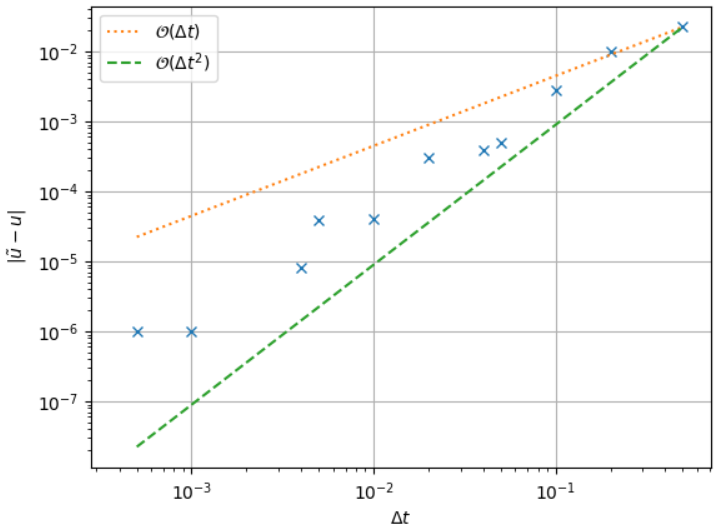
\includegraphics[width=0.5\textwidth]{resources/calculix_convergence_study.png}
        \caption{TODO: improve this figure, by adding legend and nicer colors.}
        \label{fig:calculix_convergence}
    \end{figure}

\end{itemize}

\section{Coupling the two solvers}
\begin{itemize}
    \item Talk about what a FSI is in general. Talk more specifically about the perpendicular flap case study, based on the preCICE tutorials.
    \item Talk about the automatization of this, using scripts.
    \item Supported time stepping schemes, difference between v2 and v3.
\end{itemize}
\subsection{Simulation parameters}
    \begin{itemize}
    \item Talk about the parameters of the two solvers (mainly the same as the previous simulations, except change of openFAOM solver). 
    \item Mention the possible preCICE parameters (window-size, ...).
    \end{itemize} 

\subsection{Case study: FSI - perpendicular flap}
\begin{itemize}
    \item Comment on Figure \ref{fig:coupled_v2_v3}. Show how First order convergence seems to be working, but higher order performs poorly. This is due to an error on the openFAOM adapter, which only supports Euler timestepping.
    \item Crank Nikolson needs two evaluations per time step, or reuse buffered data of previous timesteps (what is doing openFAOM, most likely, TODO: check this.).
    \item Give reasoning why this is not working, give some clues what should be done to actually improve it.
\end{itemize}


\begin{figure}[!ht]
    \centering
    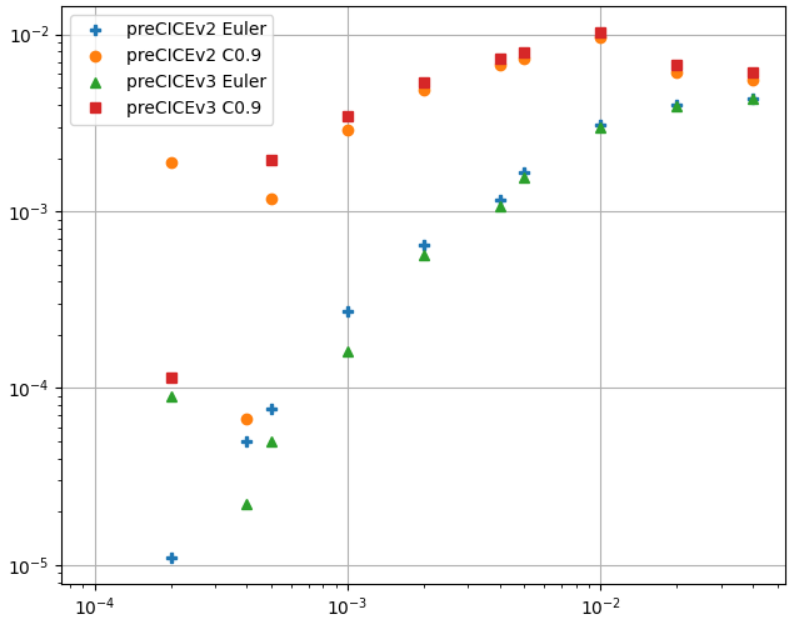
\includegraphics[width=0.5\textwidth]{resources/coupled_v2_v3_results.png}
    \caption{TODO: add title and maybe convergence lines}
    \label{fig:coupled_v2_v3}
\end{figure}


\section{OpenFOAM Adapter}
\begin{itemize}
    \item Maybe explain a bit how it interacts with the solver, quite documented already by \href{https://precice.org/adapter-openfoam-extend.html}{Adapter documentation}, and by \href{https://journal.openfoam.com/index.php/ofj/article/view/88/78}{Article of Gerasimos et al.}.
    \item Mention what should be fixed, maybe propose a prototype?
    \item Mention how should be tested, with a fake-fluid setup for example. Then also test with the same setup to see if it is viable.
\end{itemize}

\section{Conclusions and future work}
\begin{itemize}
    \item Talk about the convergence conclusions of each of the solvers. Mention the obtained results with the preCICE couplings.
    \item Give directions on what to fix of the OpenFOAM adapter, and what to be tested after the fixing implementation.

\end{itemize}

\printbibliography

\end{document}
